\chapter{Definition}\label{ch:definition}

\begin{wrapfigure}{R}{0.3\textwidth}
\centering
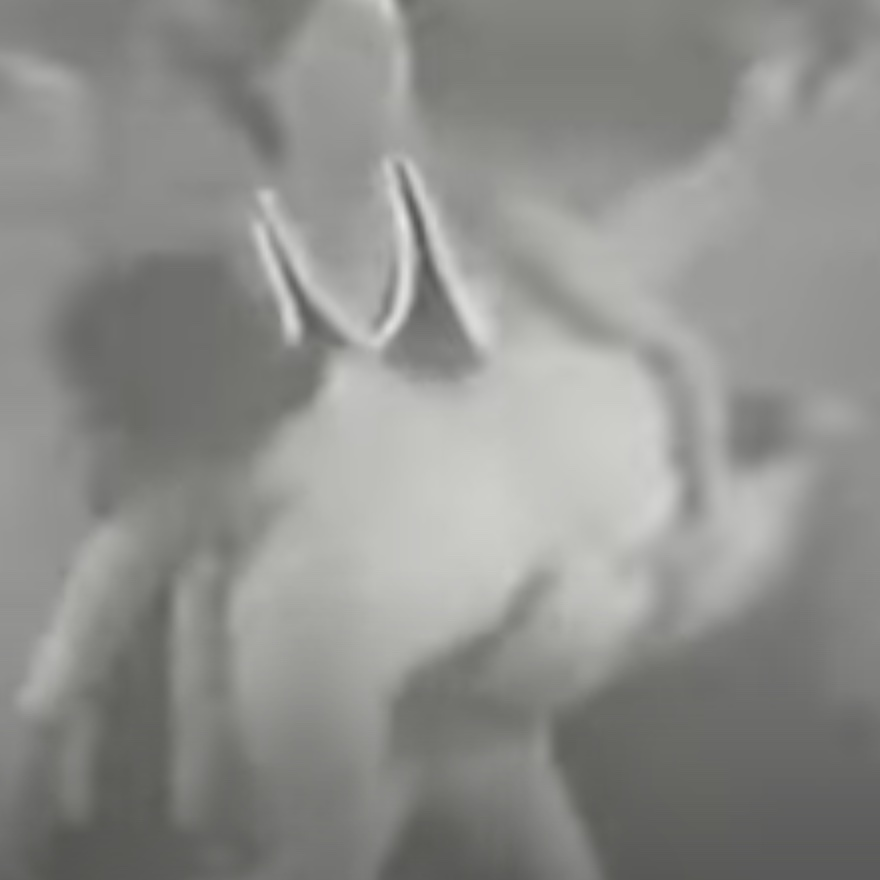
\includegraphics[width=0.25\textwidth]{images/definition}
\end{wrapfigure}

Without a proper definition of what something is, without capturing its \textbf{essence}, it can't be properly talked about.
How does it relate and especially separate itself from other similar systems?
What are its \textbf{goals and principles}, so we can always check whether a specific method or direction is in alignment with these goals and principles.
Not necessarily that it would be wrong, but just to be aware when we step out of our system, and step into something (completely) different.
Communication usually is loaded with \textbf{misunderstandings}, and by having a clear, mutual understanding of what it is we are actually referring to, we can create more \textbf{harmony} in our interaction through clarity (of words).

So what is CI (sometimes also called ``\textit{contact}'' or ``\textit{contact dance}'' in the community) \textbf{compared} to other systems?
A dance, a sport, a (visceral) art-form or art-sport, partner acrobatics or martial arts?
Well, maybe all of it or none of it; or maybe depending on how you approach it and what your background is and where you put the emphasis on.
Let's have a look at the different views on it, and by also looking at its history it might get more clear what it is, or what it can be for you.

\section{By Comparison}\label{sec:by-comparison}
%%%%%%%%%%%%%%%%%%%%%%%%%%%%%%%%%%%%%%%%%%%%%%%%%%%%%%%%%%%%%%%%%%%%%%%%%%%%%%%%%%%%%%%%%%%%%%%%%%%%%%%%%%%%%%%%%%%%%%%%

Most of the emphasis is put on the following areas:

\begin{itemize*}
	\item [] \textbf{Experimental dance} -- practice-based research in dance laboratories
	\item [] \textbf{Theatrical form} -- improvised performances and lectures-demonstrations
	\item [] \textbf{Educational tool} -- training for professional dancers in improvisation
	\item [] \textbf{Awareness practice} -- being able to listen to the subtleties in contact
	\item [] \textbf{Social dancing} -- at informal gatherings called ``jams''
\end{itemize*}

At its core it involves \textbf{mindfulness}, sensing and collecting information which requires full presence and attention.
And yes, it is even related to other improvisation practices like improvisation acting: the ``Yes, and \ldots''-concept expressed just physically.

\subsection{Dance}\label{subsec:dance}

It could be considered a form of improvised partner dancing, embedded in contemporary and (post-)modern dance form.
Dance improvisation existed already before CI, but it didn't have the \textbf{contact} aspect as CI has, and most of it all the ``\textit{shared point of contact}'' principle.
The development in dance history started with ballet, to modern (Martha Gram, John Cage, Cunningham), and then towards contemporary -- improvisation became not only a research tool, but a performance itself.
Those are mostly vertically, meaning standing, without any floorwork involved; whereas in CI we roll over each other on the floor, something which would be seen as rather unusual in other styles.
We use a \textbf{three-dimensional} spherical space, were every body-part can be a foot -- and be pushed against the ground.

CI is an \textbf{improvised} ``art-form'' (or ``art-sport''), thus without any predefined choreography.
Sometimes CI is used in choreographies, which is then called ``partnering''.
CI is an exploration, a way to try to ``break the system'' as it is improvised.
Nevertheless, CI is not something you would see in the professional dance world, a world where they are walking with very ``nice movements''.

It is not so much that as a CI dancer you are serving the \textbf{audience} (in a performance), but rather that the audience is joining you.
It's about getting a visceral reaction from the audience of an improvisation art-form, that they want to join.
Ultimately there is no difference between dancers and the audience, no hierarchy is existing.

It is distinct from other partner dance styles, as those are more focused on the social aspect, whereas CI comes from the art world.
Many other dances are also very much \textbf{gender-roled}, where usually the man would lead, and the woman would follow (exceptions exist like for example Lindy Hop).
In CI, everyone dances with everyone, without any clearly defined role.

CI has a strong focus on the \textbf{physical} aspect: How to survive a high impact volume, which leads to either to crash or to fall?
Lindy Hop is for example also very strong in acrobatics, which Zouk also does a little.
Thinking about taking/lifting people on your body, on your core, your center.

There is also a difference in styling, as many \textbf{aesthetically} pleasing dance styles would ``dress to impress''.
In CI, we would typically come wearing our pyjamas, sloppy, cosy, comfy, pragmatic.

\subsection{Martial Art}\label{subsec:martial-art}

It is also combined with some minor aspects of eastern philosophy and a few things from the 1960s hippie culture.
Reason being that some founders of CI had their background in the Japanese martial art of \textbf{Aikido}, which is similar to Brazilian Jiu Jitsu.
Gently receiving incoming force and deflect it in circular movements, not resisting but rather listen, perceive, interpret and work with what's there at the moment.

Yet of course CI totally lacks the intention of it being even remotely applied in a contest or let alone in a street fight.
There is no emphasize put on practicality during a physical conflict, still having skills in for example rolling (Judo) can be extremely handy.

\subsection{Applied Physics}\label{subsec:applied-physics}

CI is an exploration of \textbf{physical forces} of one's body in relationship to others by using the principle of sharing weight, touch, and movement awareness, while moving in contact and on the ground.
To play with the artistry of falling off balance and counterbalance, with gravity and physics.
To learn the mechanics of the body to handle someone's weight or to be lifted, along with breathing techniques.
Alternatively it can be stated:

\begin{center}
	``\textit{CI is a three-body-problem with two dancers, being shaped/moved by momentum, gravity, and force, dealing with the third body, the ground/earth.}''
\end{center}

\subsection{Acrobatics}\label{subsec:acrobatics}

The main founder, Steve Paxton himself was a \textbf{gymnast}, and that might be the reason why still some of CI resembles more partner acrobatics than dancing.
The many (demanding) lifts, and the high velocity and high impact movements can require a high level of fitness of the practitioners, just like acrobatics does.
Whereas proper partner acrobatics goes way beyond what CI is doing, in terms of physical demands and risky techniques.

\section{Community}\label{sec:community}
%%%%%%%%%%%%%%%%%%%%%%%%%%%%%%%%%%%%%%%%%%%%%%%%%%%%%%%%%%%%%%%%%%%%%%%%%%%%%%%%%%%%%%%%%%%%%%%%%%%%%%%%%%%%%%%%%%%%%%%%

The term ``community'' is in some areas used for people living in the same place, something hippies would do who strive for a more ``natural'' approach to life, people who drop out the system, sharing knowledge about each other, rather than about a specific \textbf{practice}, and helping each other in times of need.
And there is even a current trend in our society that companies are using phrases like ``Come, join the family!'' which even deludes the word family very much.

We use the term ``community'' here for a group of people \textbf{sharing} the same passion for this practice, and getting curious about the other person, from a very basic physical connection.
Sometimes this curiosity goes to their life, experiences, and ideas, which sometimes can lead to afterward also sharing food; from their, friendship can happen.
Sometimes it is also just a great dance partner, but personally we might have nothing in common, and we also do not want to become friends.
We see each other as ``only dance partners'', and the depth of care we feel is a bit less than for example for our beloved neighbour.

In the CI ``community'' this is a bit off though (compared to regular dance scenes), as when someone discontinues to come to classes or jams after a while, we might not be real friends, yet we would still reach out for each other, asking where he is, \textbf{helping} each other out (with health issues, financially) and support if needed.
This happens especially in smaller classes, where there is more of a sense of community.
These silos also happen according to the attitude of the teacher or the jam, where people will converge into specific places; norms will differ based on that.

People who practice or teach CI believe in what they do, in the goodness that it gives the world.
They want to expand the pool to reach more people; and that's why you will see little competition and more \textbf{collaboration} in the scene.
Maybe there will be a bit more competition if it's one's only source of income, a scarce modality; instead of CI being a livelihood, a hobby, a passion.
Some teachers will invite guest teachers, or send their students to another teacher, to a different city, or a teacher who is more technical or in some other way different.
There is not much ``fighting'' among CI practitioners happening, but also collaboration are not so often happening, as it is a very \textbf{individual practice}.
There are festivals, where (abroad) teachers are being invited, but usually when invited, then not by other teachers but by schools, institutions, or organizers.
The norm is nevertheless a ``city-based'' teacher who offers 2--3 classes a week, and sometimes there are ``travelling teachers''.
And there is also a win-win-win in having different student-teacher relationships in one's own workshop.

\section{Stereotype}\label{sec:stereotype}
%%%%%%%%%%%%%%%%%%%%%%%%%%%%%%%%%%%%%%%%%%%%%%%%%%%%%%%%%%%%%%%%%%%%%%%%%%%%%%%%%%%%%%%%%%%%%%%%%%%%%%%%%%%%%%%%%%%%%%%%

There is no clear stereotypical, \textbf{physical appearance} for so-called ``CI people'', as we might have when thinking of people who do Yoga, Hip Hop, or Tantra.
CI practitioners are nevertheless very quickly spotted on the dance floor, not so much based on their looks but how they move, how they engage, their behavior with weight.
There seems to be a mutual, unconscious ability to spot each other on the dance floor which makes them find each other rather quickly -like magic.

A stereotypical CI practitioner is often wearing common \textbf{dance clothes}, nothing too casual or street clothes, but also nothing too fancy.
The age range is rather big, yet for the technical part it's usually around 25--45.
Socioeconomically it's a little bit on the higher end, meaning people who are \textbf{financially} a bit better off.
Teachers might be willing to give a discount to people who cant easily afford paying for the classes/workshops, so in case needed, feel free to go ahead and ask, as the worst thing you could get is a ``no'' and in the best case you can afford going for your dream.
Also, strictly \textbf{religious} people seem not to be attracted by it, most likely because of the touch and the physical proximity.

CI people have no need to attach themselves to a \textbf{subculture} and shape their personality around it; there is no need for ``another stamp'' as is seen so often in other practices.
CI is about the \textbf{physicality}, and less a ``spiritual practice for personal growth'', or a community, as stated above.
Still, the way we move might influence our personality; similar to the increased sensuality when moving Tango, but that's not a big thing in CI\@.
It's very \textbf{egalitarian}, meaning no roles, and a plain physical form.
It's more \textbf{technical}, more raw, and no (moral) values are being conveyed -whereas the egalitarian approach might be a value in itself.
It is \textbf{independent} of sex, gender, age, and body; there is no leading nor following based on sex or gender -just play.
It doesn't convince others of they greatness of CI, although everyone is invited and welcome to join -it's fun.

\section{Jams}\label{sec:jams}
%%%%%%%%%%%%%%%%%%%%%%%%%%%%%%%%%%%%%%%%%%%%%%%%%%%%%%%%%%%%%%%%%%%%%%%%%%%%%%%%%%%%%%%%%%%%%%%%%%%%%%%%%%%%%%%%%%%%%%%%

There is a broad, global community which organizes social dances, so-called ``jams'', on a regular basis and practitioners often overlap with the Ecstatic Dance \footnote{Many people from Ecstatic Dance often claim to have done ``contact'' but actually have no idea about CI. This confusion is about ``touch based partner dance'' versus the art-form of CI (sharing weight). These people might also bring in a slight different (sensual-sexual, maybe even Tantric) attitude which is not welcome in CI.} communities.
They are \textbf{social gatherings} without a leader, yet sometimes with someone who facilitates it; similar to jazz jam sessions or Milongas in Tango.
It's an opportunity to practice \textbf{freely}, where people can meet and negotiate together their dance, or observe the practice of their partners.
It's an occasions to meet other fellow practitioners, friends or strangers, old, young, experienced, and novice.
It's a hybrid between bodily meditation, psycho-kinesthetic therapy, sports training and a dance improvised session.
They can be regularly in a studio for a few hours, or longer retreat jams for several days in spring resorts where it can be practiced at any hour of the day.

Sometimes you will encounter that the \textbf{facilitator} takes a bit more the lead, by hosting sharing circles at the beginning and/or at the end, and by providing some warm-up exercises.
Sometimes you will have a playlist providing musical background throughout, sometimes you might even encounter a live musician.
Yet, traditionally jams are being kept \textbf{silent}; to let fully unfold of what is alive at the moment between the dancing partners; to not let the music dictate externally but allow for full expression of what's present, as one of my dance teachers once said: ``\textit{Music makes a dancer stupid}''.

At the end (also sometimes in classes/workshops), you will sometimes find that people engage in an exercise called ``\textbf{round-robin}'', which means that a few couples (or half of the people) are constantly in the center of the room, all the other people sitting on the edge holding space, being present, observing and learning or at least get inspired, giving in their energy, and when you enter/join a couple, another person is leaving, so the amount of people stays constant throughout.

\section{Historically}\label{sec:historically}
%%%%%%%%%%%%%%%%%%%%%%%%%%%%%%%%%%%%%%%%%%%%%%%%%%%%%%%%%%%%%%%%%%%%%%%%%%%%%%%%%%%%%%%%%%%%%%%%%%%%%%%%%%%%%%%%%%%%%%%%

In the early beginnings, in the 1970s, everytime the founding members practiced CI, they would redefine it, asking the veru same question over and over again: ``What is CI \textit{now}?'' An early definition by \textbf{Steve Paxton} and others was (source: CQ Vol. 5:1, Fall 1979):

\begin{displayquote}
``A continuously evolving system of improvised movement.
Two bodies, communicating with each other in physical contact, creating a relationship with the physical laws (motion, gravity, momentum, inertia).
Sensitive, thus relaxed of unnecessary muscular tension, and willing to experience a natural flow.
Techniques may include: Rolling, falling, being upside down, following, supporting and giving weight.

A physical dialogue ranging from stillness to highly energetic exchange.
Alert enough to stay in an energetic state of physical disorientation, trusting your survival instincts.
A free play seeking for balanced movements, leading to a physical and emotional truth, shared at the moment, leaving you informed, centered, and enlivened.''
\end{displayquote}

\section{Possible Definitions}\label{sec:possible-definitions}
%%%%%%%%%%%%%%%%%%%%%%%%%%%%%%%%%%%%%%%%%%%%%%%%%%%%%%%%%%%%%%%%%%%%%%%%%%%%%%%%%%%%%%%%%%%%%%%%%%%%%%%%%%%%%%%%%%%%%%%%

Definitions, and the same with any terminology, are time-, space- and person-dependent.
Just as with the improvised nature of CI, it is a constantly moving target.
By asking the same question a week later, the answer you receive will already be different.

There is still a rough \textbf{body of agreement} -- a congruent understanding -- of what it is, and what it is not, leading to a definition stable across time, space, and practitioner.
It's like a tree: The trunk which are the agreed principles, and it's branches and leaves (the styles/adaptations) representing the edges where you can play freely.

\textbf{Steve Paxton} himself stated in 1979:
\begin{displayquote}
	``The exigencies\footnote{exigency = A pressing or urgent situation/requirement/need.} of the form dictate a mode of movement which is relaxed, constantly aware and prepared, and onflowing.
	As a basic focus, the dancers remain in physical touch, mutually supportive and innovative, meditating upon the physical laws relating to their masses: gravity, momentum, inertia, and friction.
	They do not strive to achieve results, but rather, to meet the constantly changing physical reality with appropriate placement and energy.''
\end{displayquote}

\textbf{Nancy Start Smith} once mentioned:
\begin{displayquote}
	``It resembles other familiar duet forms, such as the embrace, wrestling, surfing, martial arts, and the Jitterbug (Lindy Hop and swing dances), encompassing a wide range of movement from stillness to highly athletic.''
\end{displayquote}

\textbf{Daniel Lepkoff} states about the core of CI:
\begin{displayquote}
	``To put focus on bodily awareness and physical reflexes, rather than consciously controlled movements.
	Precedence of body experience first, and mindful cognition second, is an essential distinction between CI and other approaches to dance.''
\end{displayquote}

\textbf{Ray Chung} once announced in a workshop 2009 that:
\begin{displayquote}
	CI is an open-ended exploration of the kinaesthetic possibilities of bodies moving through contact.
	Sometimes wild and athletic, sometimes quiet and meditative, it is a form open to all bodies and enquiring minds.
\end{displayquote}

\section{Beyond CI}\label{sec:beyond-ci}
%%%%%%%%%%%%%%%%%%%%%%%%%%%%%%%%%%%%%%%%%%%%%%%%%%%%%%%%%%%%%%%%%%%%%%%%%%%%%%%%%%%%%%%%%%%%%%%%%%%%%%%%%%%%%%%%%%%%%%%%

CI is for sure not a pure \textbf{martial art}, as it has no claim to have any practical fighting application.
Nor is it a competitive \textbf{sport} in any way, as there are no competitions and due to its artistic nature it would be difficult, or at least without much meaning, to judge one as being better than the other.
It has many aspects of partner \textbf{acrobatics}, but lacks many technical possibilities due to the nature of its principles.

It is also not really your regular \textbf{dance} form like Salsa or Tango, due to several reasons: We don't dress (nor dance) to impress but rather show up with our authentic selves; we don't move in order to look good or aesthetically (to others); we focus more on the internal and interpersonal aspects than the external ones; we dance often without music; there are no real techniques which can be learned but only guiding principles from which some specific movements can emerge.

As it is the case with so many (or maybe even all?) disciplines: Once the rule has been understood, and you know what you are doing, it can be broken by the student, thus \textbf{becoming a master} of it.
Finally, it has to be mentioned that a system\footnote{In this case we talk about CI as a system, but the forementioned wisdome can be applied to our world's system, politically or economically, to technology, to our endless todo lists \ldots} is supposed to be of service to the user (not the other way round), and its boundaries and dogma should not limit but enrich the applicant.
Whenever the purpose is hindered by the system, the system shall be left behind, and we should remember the original goal which was there in the first place, and not to serve the gods we created.
